% This file was created by tikzplotlib v0.8.7.
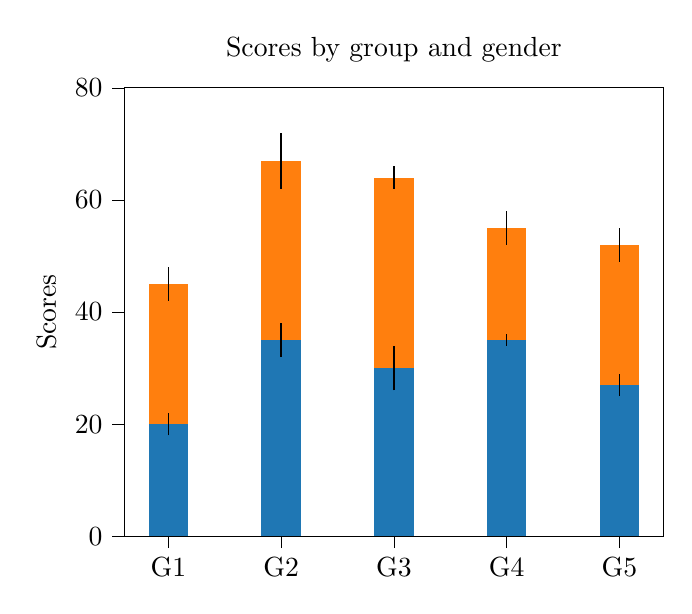
\begin{tikzpicture}

\definecolor{color0}{rgb}{0.12156862745098,0.466666666666667,0.705882352941177}
\definecolor{color1}{rgb}{1,0.498039215686275,0.0549019607843137}

\begin{axis}[
legend cell align={left},
legend style={fill opacity=0.8, draw opacity=1, text opacity=1, draw=white!80.0!black},
tick align=outside,
tick pos=left,
title={Scores by group and gender},
x grid style={white!69.01960784313725!black},
xmin=-0.3925, xmax=4.3925,
xtick style={color=black},
xtick={0,1,2,3,4},
xticklabels={G1,G2,G3,G4,G5},
y grid style={white!69.01960784313725!black},
ylabel={Scores},
ymin=0, ymax=80,
ytick style={color=black}
]
\draw[fill=color0,draw opacity=0] (axis cs:-0.175,0) rectangle (axis cs:0.175,20);
\draw[fill=color0,draw opacity=0] (axis cs:0.825,0) rectangle (axis cs:1.175,35);
\draw[fill=color0,draw opacity=0] (axis cs:1.825,0) rectangle (axis cs:2.175,30);
\draw[fill=color0,draw opacity=0] (axis cs:2.825,0) rectangle (axis cs:3.175,35);
\draw[fill=color0,draw opacity=0] (axis cs:3.825,0) rectangle (axis cs:4.175,27);
\draw[fill=color1,draw opacity=0] (axis cs:-0.175,20) rectangle (axis cs:0.175,45);
\draw[fill=color1,draw opacity=0] (axis cs:0.825,35) rectangle (axis cs:1.175,67);
\draw[fill=color1,draw opacity=0] (axis cs:1.825,30) rectangle (axis cs:2.175,64);
\draw[fill=color1,draw opacity=0] (axis cs:2.825,35) rectangle (axis cs:3.175,55);
\draw[fill=color1,draw opacity=0] (axis cs:3.825,27) rectangle (axis cs:4.175,52);
\path [draw=black, semithick]
(axis cs:0,18)
--(axis cs:0,22);

\path [draw=black, semithick]
(axis cs:1,32)
--(axis cs:1,38);

\path [draw=black, semithick]
(axis cs:2,26)
--(axis cs:2,34);

\path [draw=black, semithick]
(axis cs:3,34)
--(axis cs:3,36);

\path [draw=black, semithick]
(axis cs:4,25)
--(axis cs:4,29);

\path [draw=black, semithick]
(axis cs:0,42)
--(axis cs:0,48);

\path [draw=black, semithick]
(axis cs:1,62)
--(axis cs:1,72);

\path [draw=black, semithick]
(axis cs:2,62)
--(axis cs:2,66);

\path [draw=black, semithick]
(axis cs:3,52)
--(axis cs:3,58);

\path [draw=black, semithick]
(axis cs:4,49)
--(axis cs:4,55);

\end{axis}

\end{tikzpicture}
